\subsection{Program slave GBTx with configuration files}
Configure the parameter as shown in \autoref{fig:gbt-file}.

\begin{figure}[ht]
	\centering
    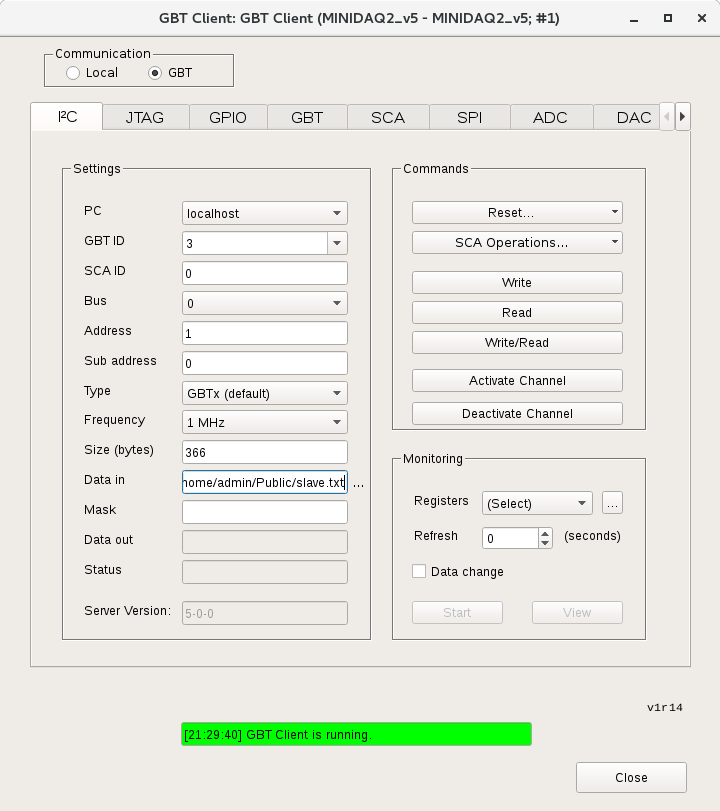
\includegraphics[width=0.9\textwidth]{res/gbt_client_slave_program_via_config_file.png}
	\caption{Parameters to program slave GBTx with a configuration file.}
	\label{fig:gbt-file}
\end{figure}

The configuration file should be supplied to the \textbf{Data in} field with the
following syntax:
\begin{minted}[frame=single]{powershell}
file:<path_to_configuration_file>
\end{minted}

The actual configuration file, depends on whether the slave is configured in
transmitter or transceiver mode, is located at:
\begin{minted}[frame=single]{powershell}
/home/admin/Public/slave-{Tx,TRx}.txt
\end{minted}

\begin{leftbar}
    This is equivalent to program the slave with an external \itwoc adapter.
    The advantage of doing this way is we don't need to remove the \itwoc
    adapter from the master.
    In other words, once the hardware setup is done, we don't have to touch them
    anymore; whereas if we program both master and slave with an \itwoc adapter,
    it must be moved around between the master and the slave.
\end{leftbar}
